%--------------------------------------------------------------------------------------------------%
\chapter{IMPLEMENTASI}
\label{chap:4}
%--------------------------------------------------------------------------------------------------%

Bab ini berisi penjelasan spesifik proses implementasi pada setiap tahap. Secara garis besar
implementasi Lex2KG terdiri dari OCR, pemindaian menjadi \textit{span}, membersihkan \textit{span},
\textit{parsing span} menjadi komponen, deteksi rujukan, dan konstruksi. Selain itu dibahas juga
mengenai bagaimana kualitas konversi dipertahankan dan bagaimana melakukan SPARQL \textit{query}
untuk melakukan evaluasi. Seluruh algoritma dan program yang digunakan dijelaskan secara rinci dalam
bab ini. Seluruh program dan \textit{resource} tersedia pada repositori
Lex2KG.\footnote{\url{https://github.com/aabccd021/legal-kg}}

%--------------------------------------------------------------------------------------------------%
\section{\textit{Maintained PDFs}}
\label{sec:maintained-pdfs}
%--------------------------------------------------------------------------------------------------%

\textit{Maintained PDFs} merupakan berkas-berkas PDF \legal yang akan di-\textit{maintain} kualitas
konversinya. Pengembangan sistem konversi dilakukan secara iteratif, dan setiap terjadi perubahan
pada sistem konversi, akan diperiksa apakah untuk semua \textit{maintained PDFs} memberikan hasil
konversi dengan kualitas yang tinggi. Pemeriksaan hasil konversi dilakukan secara manual dengan
melihat satu per satu \textit{diff} dari hasil konversi. Berikut adalah daftar peraturan
\textit{maintained PDFs}.

\begin{itemize}
  \item Peraturan Daerah Provinsi Jakarta Nomor 2 Tahun 2020 tentang Penanggulangan Corona Virus Disease 2019
  \item Peraturan Gubernur DKI Jakarta Nomor 33 Tahun 2020 tentang Pelaksanaan Pembatasan Sosial Berskala Besar dalam Penanganan Corona Virus Disease 2019 (Covid-19) Di Provinsi Daerah Khusus Ibukota Jakarta
  \item Peraturan Gubernur DKI Jakarta Nomor 3 Tahun 2021 tentang Peraturan Pelaksanaan Peraturan Daerah Nomor 2 Tahun 2020 tentang Penanggulangan Corona Virus Disease 2019
  \item Peraturan Walikota Malang Nomor 19 Tahun 2020 tentang Pedoman Penerapan Masyarakat Produktif dan Aman Covid-19
  \item Peraturan Pemerintah Nomor 74 Tahun 2020 tentang Lembaga Pengelola Investasi
  \item Peraturan Pemerintah Nomor 34 Tahun 2021 tentang Penggunaan Tenaga Kerja Asing
  \item Undang-Undang Nomor 12 Tahun 1997 tentang Perubahan atas Undang-Undang Nomor 6 Tahun 1982 tentang Hak Cipta sebagaimana Telah Diubah dengan Undang-Undang Nomor 7 Tahun 1987
  \item Undang-Undang Nomor 13 Tahun 2003 tentang Ketenagakerjaan
  \item Undang-Undang Nomor 6 Tahun 2018 tentang Kekarantinaan Kesehatan
  \item Undang-Undang Nomor 1 Tahun 2020 tentang Pengesahan Persetujuan Kemitraan Ekomomi
  Komprehensif Indonesia-Australia (Indonesia-Australia Comprehensive Economic Partnership
  Agreement)
  \item Undang-Undang Nomor 11 Tahun 2020 tentang Cipta Kerja
\end{itemize}

%--------------------------------------------------------------------------------------------------%
\section{OCR Ulang Berkas PDF}
\label{sec:ocr-ulang-berkas-pdf}
%--------------------------------------------------------------------------------------------------%

Dokumen \legal yang digunakan pada penelitian didapatkan dalam format berkas PDF. Penulis pada
awalnya mencoba langsung mengekstraksi data dari PDF, tetapi penulis menemukan kesulitan. Salah satu
kesulitan yang penulis temui adalah terdapatnya salah pemindaian pada berkas PDF. Sebagai contoh,
terdapat teks yang tertulis \mono{Pasal} tetapi mengandung data \mono{Pasai}. Selain itu, penulis
juga menemukan bahwa setiap dokumen mengandung keslahan pemindaian yang bervariasi. Untuk suatu
kasus, teks \mono{(2)} selalu terdeteksi sebagai \mono{(21} pada suatu dokumen, tetapi tidak pada
dokumen lainnya. Pada kasus lainnya terdapat dokumen yang hampir tidak memiliki kesalahan pemindaian
dan juga terdapat dokumen yang teksnya tidak dapat dibaca samasekali.

Walaupun dokumen-dokumen tersebut di-\textit{maintain} oleh satu lembaga pada satu situs web, yaitu oleh Dewan
Perwakilan Rakyat pada situs web \url{https://dpr.go.id/jdih}, masing-masing dokumen dibuat menjadi
berkas PDF dengan cara yang berbeda-beda. Penulis tidak dapat mengetahui secara pasti metode apa
yang digunakan, tetapi dari metadata yang didapatkan dari berkas PDF, penulis dapat membuat beberapa
dugaan. Pada berkas PDF, terdapat metadata dengan nama \textbf{Creator}, di mana pada
dokumen-dokumen \legal yang didapatkan, tercantum nama-nama alat pencetak atau
merk dari pencetak tersebut. Dari informasi tersebut penulis menduga bahwa terdapat sebagian
\legal yang dibuat menjadi PDF dengan mencetaknya menjadi kertas terlebih
dahulu kemudian dipindai oleh pemindai dan sebagian lainnya dikonversi langsung dari berkas
\textit{.docx}. Data yang dipindai adalah berupa gambar, artinya teks yang terdapat pada berkas PDF
adalah hasil OCR (\textit{optical character recognition}) oleh pemindai tersebut.
\tab~\ref{tab:metadata-pdf} adalah salah satu contoh dokumen beserta data yang tercantum sebagai
\textbf{Creator} dan contoh kesalahan pemindaiannya yang banyak terjadi.

\begin{table}
  \centering
  \begin{tabular}{|l|l|l|}
    \hline
    Dokumen    & \_\_Creator\_\_        & Kesalahan pemindaian        \\ \hline \hline
    UU 13/2003 & ScanSoft PDF Create! 4 & - (tidak ada)               \\ \hline
    UU 6/2018  & Canon                  & `(2)` selalu dipindai `(21` \\ \hline
    PP 34/2021 & Fuji Xerox B9100       & data teks tidak terbaca     \\ \hline
  \end{tabular}
  \caption{Metadata PDF \legal}
  \label{tab:metadata-pdf}
\end{table}

Pemindaian berkas PDF dengan metode yang berbeda-beda memberikan kualitas hasil pemindaian yang
berbeda-beda dan kesalahan pemindaian yang tidak konsisten. Untuk menyelesaikan masalah ini, penulis
melakukan OCR ulang terhadap semua dokumen yang akan dikonversi. Dengan melakukan OCR ulang
menggunakan satu metode yang sama, penulis tidak hanya berhasil mendapatkan data hasil pemindaian
berkas PDF dengan kualitas pemindaian yang konsisten untuk semua dokumen. Penulis memilih
menggunakan Tesseract OCR\footnote{\url{https://github.com/tesseract-ocr/tesseract}} sebagai metode
OCR karena sifatnya \textit{open source} dan mendukung Bahasa Indonesia sebagai bahasa yang
dipindai. Tesseract OCR merupakan mesin OCR yang awalnya dikembangkan oleh Hewlett-Packard yang
kemudian dibuka sebagai \textit{open source} dan saat ini dilanjutkan pengembangannya oleh Google.
Tesseract OCR juga dianggap \textit{open soure} OCR paling akurat saat ini.

\lst~\ref{lst:run-ocr} merupakan \textit{command} untuk melakukan konversi \mono{UU-2021-34.pdf}
yang sudah ada menjadi \mono{UU-2021-34\_OCR.pdf} hasil OCR. Opsi \mono{--force-ocr} diperlukan
untuk melakukan OCR ulang pada berkas PDF yang sudah memiliki teks hasil OCR untuk di
\textit{overwrite}. Opsi \mono{--jobs 4} menjalankan \textit{command} dengan 4 \textit{core} CPU,
bilangan pada opsi ini dapat diganti sesuai kebutuhan. Opsi \mono{--tesseract-config
tesseract-config.cfg} menjalankan \textit{command} dengan konfigurasi yang diberikan. Pada
penelitian ini, penulis menggunakan Tesseract OCR versi 4.0.

\begin{listing}[H]
  \begin{minted}[fontsize=\scriptsize, frame=single, breaklines]{text}
ocrmypdf -l ind --force-ocr --jobs 4 --tesseract-config tesseract-config.cfg UU-2021-34.pdf
UU-2021-34_OCR.pdf 
  \end{minted}
  \caption{Command untuk menjalankan OCR}
  \label{lst:run-ocr}
\end{listing}

Konfigurasi Tesseract OCR yang digunakan adalah \mono{tessedit\_pageseg\_mode 4} seperti yang
terlihat pada isi file konfigurasi pada \lst~\ref{lst:konfigurasi-ocr}. \mono{tessedit\_pageseg\_mode 4} digunakan agar
Tesseract OCR mendeteksi teks sebagai \textit{block}, bukan \textit{word} atau \textit{character}.

\begin{listing}[H]
  \begin{minted}[fontsize=\scriptsize, frame=single]{text}
# tesseract-config.cfg
tessedit_pageseg_mode 4
  \end{minted}
  \caption{Konfigurasi Tesseract OCR}
  \label{lst:konfigurasi-ocr}
\end{listing}

%--------------------------------------------------------------------------------------------------%
\section{Pemindaian Berkas PDF menjadi \textit{Span}}
\label{pemindaian-berkas-pdf-menjadi-data-span}
%--------------------------------------------------------------------------------------------------%

Agar dapat diproses oleh program, berkas PDF perlu diolah menjadi data berupa daftar teks dan
posisinya yang selanjutnya akan disebut \textit{span}. Sebuah \textit{span} mengandung satu baris
teks. \tab~\ref{tab:data-span} adalah data yang dimiliki oleh sebuah \textit{span}. \textit{Span}
yang dikeluarkan adalah berupa \textit{span} pada masing-masing halaman, sehingga perlu dilakukan
operasi \textit{flatten} untuk menghasilkan array satu dimensi yang memuat \textit{span} dari
seluruh halaman PDF. \pic~\ref{fig:contoh-dokumen} dan \lst~\ref{lst:hasil-pemindaian}
berturut-turut adalah contoh gambaran berkas PDF dan hasil pemindaiannya menjadi daftar
\textit{span}.

\begin{table}
  \centering
  \begin{tabular}{|l|l|} \hline
    Nama             & Deskripsi                                   \\\hline \hline
    \texttt{str}     & teks yand dikandung                         \\\hline
    \texttt{xL}      & koordinat titik terkiri dari \textit{span}  \\\hline
    \texttt{xR}      & koordinat titik terkanan dari \textit{span} \\\hline
    \texttt{y}       & koordinat titik teratas dari \textit{span}  \\\hline
    \texttt{pageNum} & nomor halaman                               \\\hline
    \texttt{id}      & \textit{identifier} unik untuk setiap span  \\\hline
  \end{tabular}
  \caption{Data \textit{span}}
  \label{tab:data-span}
\end{table}

\begin{figure}[H]
  \centering
  \fbox{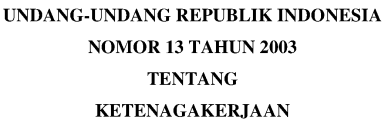
\includegraphics{pictures/pdf_example.png}}
  \caption{Contoh PDF yang akan dipindai}
  \label{fig:contoh-dokumen}
\end{figure}

\begin{listing}[H]
  \begin{minted}[fontsize=\scriptsize, frame=single]{yaml}
- xL: 197.52
  xR: 442.79990000000004
  'y': 234.48000000000002
  str: UNDANG-UNDANG REPUBLIK INDONESIA
  pageNum: 1
  id: 0
- xL: 252.72
  xR: 387.6002
  'y': 255.12
  str: NOMOR 13 TAHUN 2003
  pageNum: 1
  id: 1
- xL: 291.12
  xR: 349.68048
  'y': 275.76
  str: TENTANG
  pageNum: 1
  id: 2
- xL: 257.28
  xR: 383.28015999999997
  'y': 296.4
  str: KETENAGAKERJAAN
  pageNum: 1
  id: 3
  \end{minted}
  \caption{Hasil pemindaian \pic~\ref{fig:contoh-dokumen} dalam format yaml}
  \label{lst:hasil-pemindaian}
\end{listing}

%--------------------------------------------------------------------------------------------------%
\section{Membersihkan Data tidak Relevan dari \textit{Span}}
\label{membersihkan-noise-dari-halaman}
%--------------------------------------------------------------------------------------------------%

Tidak jarang dokumen \legal mengandung data tidak relevan yang tidak ingin kita ekstraksi seperti
\textit{header} dan \textit{footer}. Pada penelitian ini, penulis menggunakan dokumen dari sumber
yang sama sehingga memiliki format yang sama, dan juga posisi \textit{header} dan \textit{footer}
yang hampir sama pada setiap dokumen.

\begin{figure}[H]
  \centering
  \fbox{
\includegraphics{pictures/pdf_header.png}}
  \caption{Contoh header}
  \label{fig:contoh-header}
\end{figure}

\pic~\ref{fig:contoh-header} adalah contoh \textit{header} yang terdapat pada setiap halaman. Dapat
dilihat bahwa \textit{header} selalu terdiri dari teks ``PRESIDEN REPUBLIK INDONESIA'' dan diikuti
oleh nomor halaman, dan selalu terletak di posisi yang hampir sama. Oleh karena itu, penulis
memeriksa teks menggunakan \textit{regex} dan posisi dari setiap \textit{span}, kemudian menghapus
\textit{span} tersebut jika terdeteksi sebagai header. \lst~\ref{lst:remove-noise} adalah kode yang
mendeteksi data tidak relevan.

\begin{listing}[H]
  \begin{minted}[fontsize=\scriptsize, fontsize=\scriptsize, frame=single]{typescript}
function isNotHeader(span: UnindexedSpan): boolean {
  const isHeader =
    y < 220 && (['PRESIDEN', 'REPUBLIK INDONESIA'].includes(str) || /- ?[0-9]+ ?-/.test(str));
  return !isHeader;
}
function isLeftFooter(span: UnindexedSpan): boolean {
  return span.y > 900 && span.xL < 45;
}

\end{minted}
  \caption{Kode untuk mendeteksi \textit{header} dan \textit{footer}}
  \label{lst:remove-noise}
\end{listing}

%--------------------------------------------------------------------------------------------------%
\section{Pembuatan \textit{Span} "Hybrid"}
\label{penggabungan-data-berkas-pdf-asli-dan-hasil-ocr-ulang}
%--------------------------------------------------------------------------------------------------%

Pada proses pemindaian berkas PDF menjadi \textit{span}, penulis menemukan satu masalah yaitu data
hasil OCR tidak konsisten dalam memindai angka. Seperti yang dapat dilihat pada
\pic~\ref{fig:contoh-nomor-tidak-terpindai}, angka 10 berhasil dipindai tetapi angka 9 tidak
berhasil. Untuk kasus tersebut, angka hanya tidak terpindai pada hasil OCR, tetapi terpindai dengan
benar pada berkas PDF aslinya. Penulis menggabungkan \textit{span} "Asli" dan \textit{span} "OCR"
untuk membuat \textit{span} "Hybrid" yang melengkapi bagian yang tidak terpindai.

\begin{figure}[H]
  \centering
  \fbox{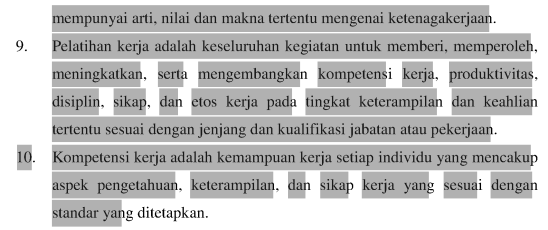
\includegraphics{pictures/pdf_unscanned_number.png}}
  \caption{Contoh nomor tidak terpindai}
  \label{fig:contoh-nomor-tidak-terpindai}
\end{figure}

Penulis hanya melakukan penggabungan \textit{span} untuk kasus angka seperti yang disebutkan di
atas. Hal tersebut dikarenakan pada umumnya kita dapat mentolerir kesalahan pemindaian pada teks,
tetapi karena kegagalan pemindaian pada angka tersebut akan mempengaruhi struktur dokumen, penulis
memutuskan solusi di atas. Sebagai contoh, jika nomor 8 berhasil dipindai dan nomor 9 tidak
berhasil, maka struktur akhir yang dihasilkan akan mengandung semua isi nomor 9 didalam nomor 8,
yang mana seharusnya adalah nomor yang terpisah. \lst~\ref{lst:no-9-tidak-terpindai} dan
\lst~\ref{lst:no-9-terpindai} berturut-turut adalah contoh data yang dihasilkan jika nomor 9 tidak
berhasil terpindai dan jika berhasil terpindai.

\begin{listing}[H]
  \begin{minted}[fontsize=\scriptsize, fontsize=\scriptsize, frame=single]{yaml}
- type: point
  key: 8
  text: >-
    Informasi ketenagakerjaan adalah gabungan, rangkaian, dan analisis data yang
    berbentuk angka yang telah diolah, naskah dan dokumen yang mempunyai arti,
    nilai dan makna tertentu mengenai ketenagakerjaan.
    9. Pelatihan kerja adalah keseluruhan kegiatan untuk memberi, memperoleh,
    meningkatkan, serta mengembangkan kompetensi kerja, produktivitas, disiplin,
    sikap, dan etos kerja pada tingkat keterampilan dan keahlian tertentu sesuai
    dengan jenjang dan kualifikasi jabatan atau pekerjaan.
\end{minted}
  \caption{Data jika nomor 9 tidak berhasil terpindai dalam format yaml}
  \label{lst:no-9-tidak-terpindai}
\end{listing}


\begin{listing}[H]
  \begin{minted}[fontsize=\scriptsize, frame=single]{yaml}
- type: point
  key: 8
  text: >-
    Informasi ketenagakerjaan adalah gabungan, rangkaian, dan analisis data yang
    berbentuk angka yang telah diolah, naskah dan dokumen yang mempunyai arti,
    nilai dan makna tertentu mengenai ketenagakerjaan.
- type: point
  key: 9
  text: >-
    Pelatihan kerja adalah keseluruhan kegiatan untuk memberi, memperoleh,
    meningkatkan, serta mengembangkan kompetensi kerja, produktivitas, disiplin,
    sikap, dan etos kerja pada tingkat keterampilan dan keahlian tertentu sesuai
    dengan jenjang dan kualifikasi jabatan atau pekerjaan.
  
\end{minted}
  \caption{Data jika nomor 9 terpindai dalam format yaml}
  \label{lst:no-9-terpindai}
\end{listing}

%--------------------------------------------------------------------------------------------------%
\section{\textit{Parsing span} menjadi Komponen}
\label{pengelompokan-span-menjadi-komponen}
%--------------------------------------------------------------------------------------------------%

% // TODO: regex2nya bs dtmbhin dan ceritain

Teks yang membentuk suatu komponen terdiri dari satu atau lebih \textit{span}, sehingga daftar
\textit{span} yang didapatkan dari hasil ekstraksi berkas PDF harus dikelompokkan sehingga setiap
kelompok merepresentasikan \textit{span} yang terdapat pada suatu komponen. Pengelompokan dilakukan
dengan mendeteksi \textit{span} awal dan \textit{span} akhir dari sebuah komponen. Karena daftar
\textit{span} hasil ekstraksi bersifat 1 dimensi, hal ini bisa dilakukan dengan melakukan iterasi
pada setiap \textit{span}, kemudian menandai awal atau akhir dari sebuah kelompok apabila memenuhi
suatu pola. Setelah ditandai, \textit{span} akan dikelompokkan sebagai daftar \textit{span} dari
suatu komponen.

Pengelompokan tidak selalu langsung dilakukan dari daftar \textit{span} menjadi komponen. Daftar
\textit{span} dapat dikelompokkan menjadi grup untuk pembagian dokumen secara garis besar, kemudian
baru dikelompokkan sebagai komponen dari masing-masing grup tersebut. Pada
\pic~\ref{fig:ilustrasi-ekstraksi} grup ditandai dengan \textcolor{blue}{warna biru} dan komponen
ditandai dengan \textcolor{red}{warna merah}. Dapat dilihat bahwa daftar \textit{span} data awal
dikelompokkan menjadi komponen \textbf{DaftarBab} dan beberapa grup yaitu \textbf{Judul},
\textbf{Metadata}, dan \textbf{Disahkan}. Kemudian \textit{span} pada grup \textbf{Metadata} dikelompokkan
menjadi komponen \textbf{Menimbang}. Pengelompokan bertingkat ini dilakukan agar fungsi untuk
mendeteksi batas antara komponen tidak menjadi rumit.

\begin{figure}[H]
  \centering
  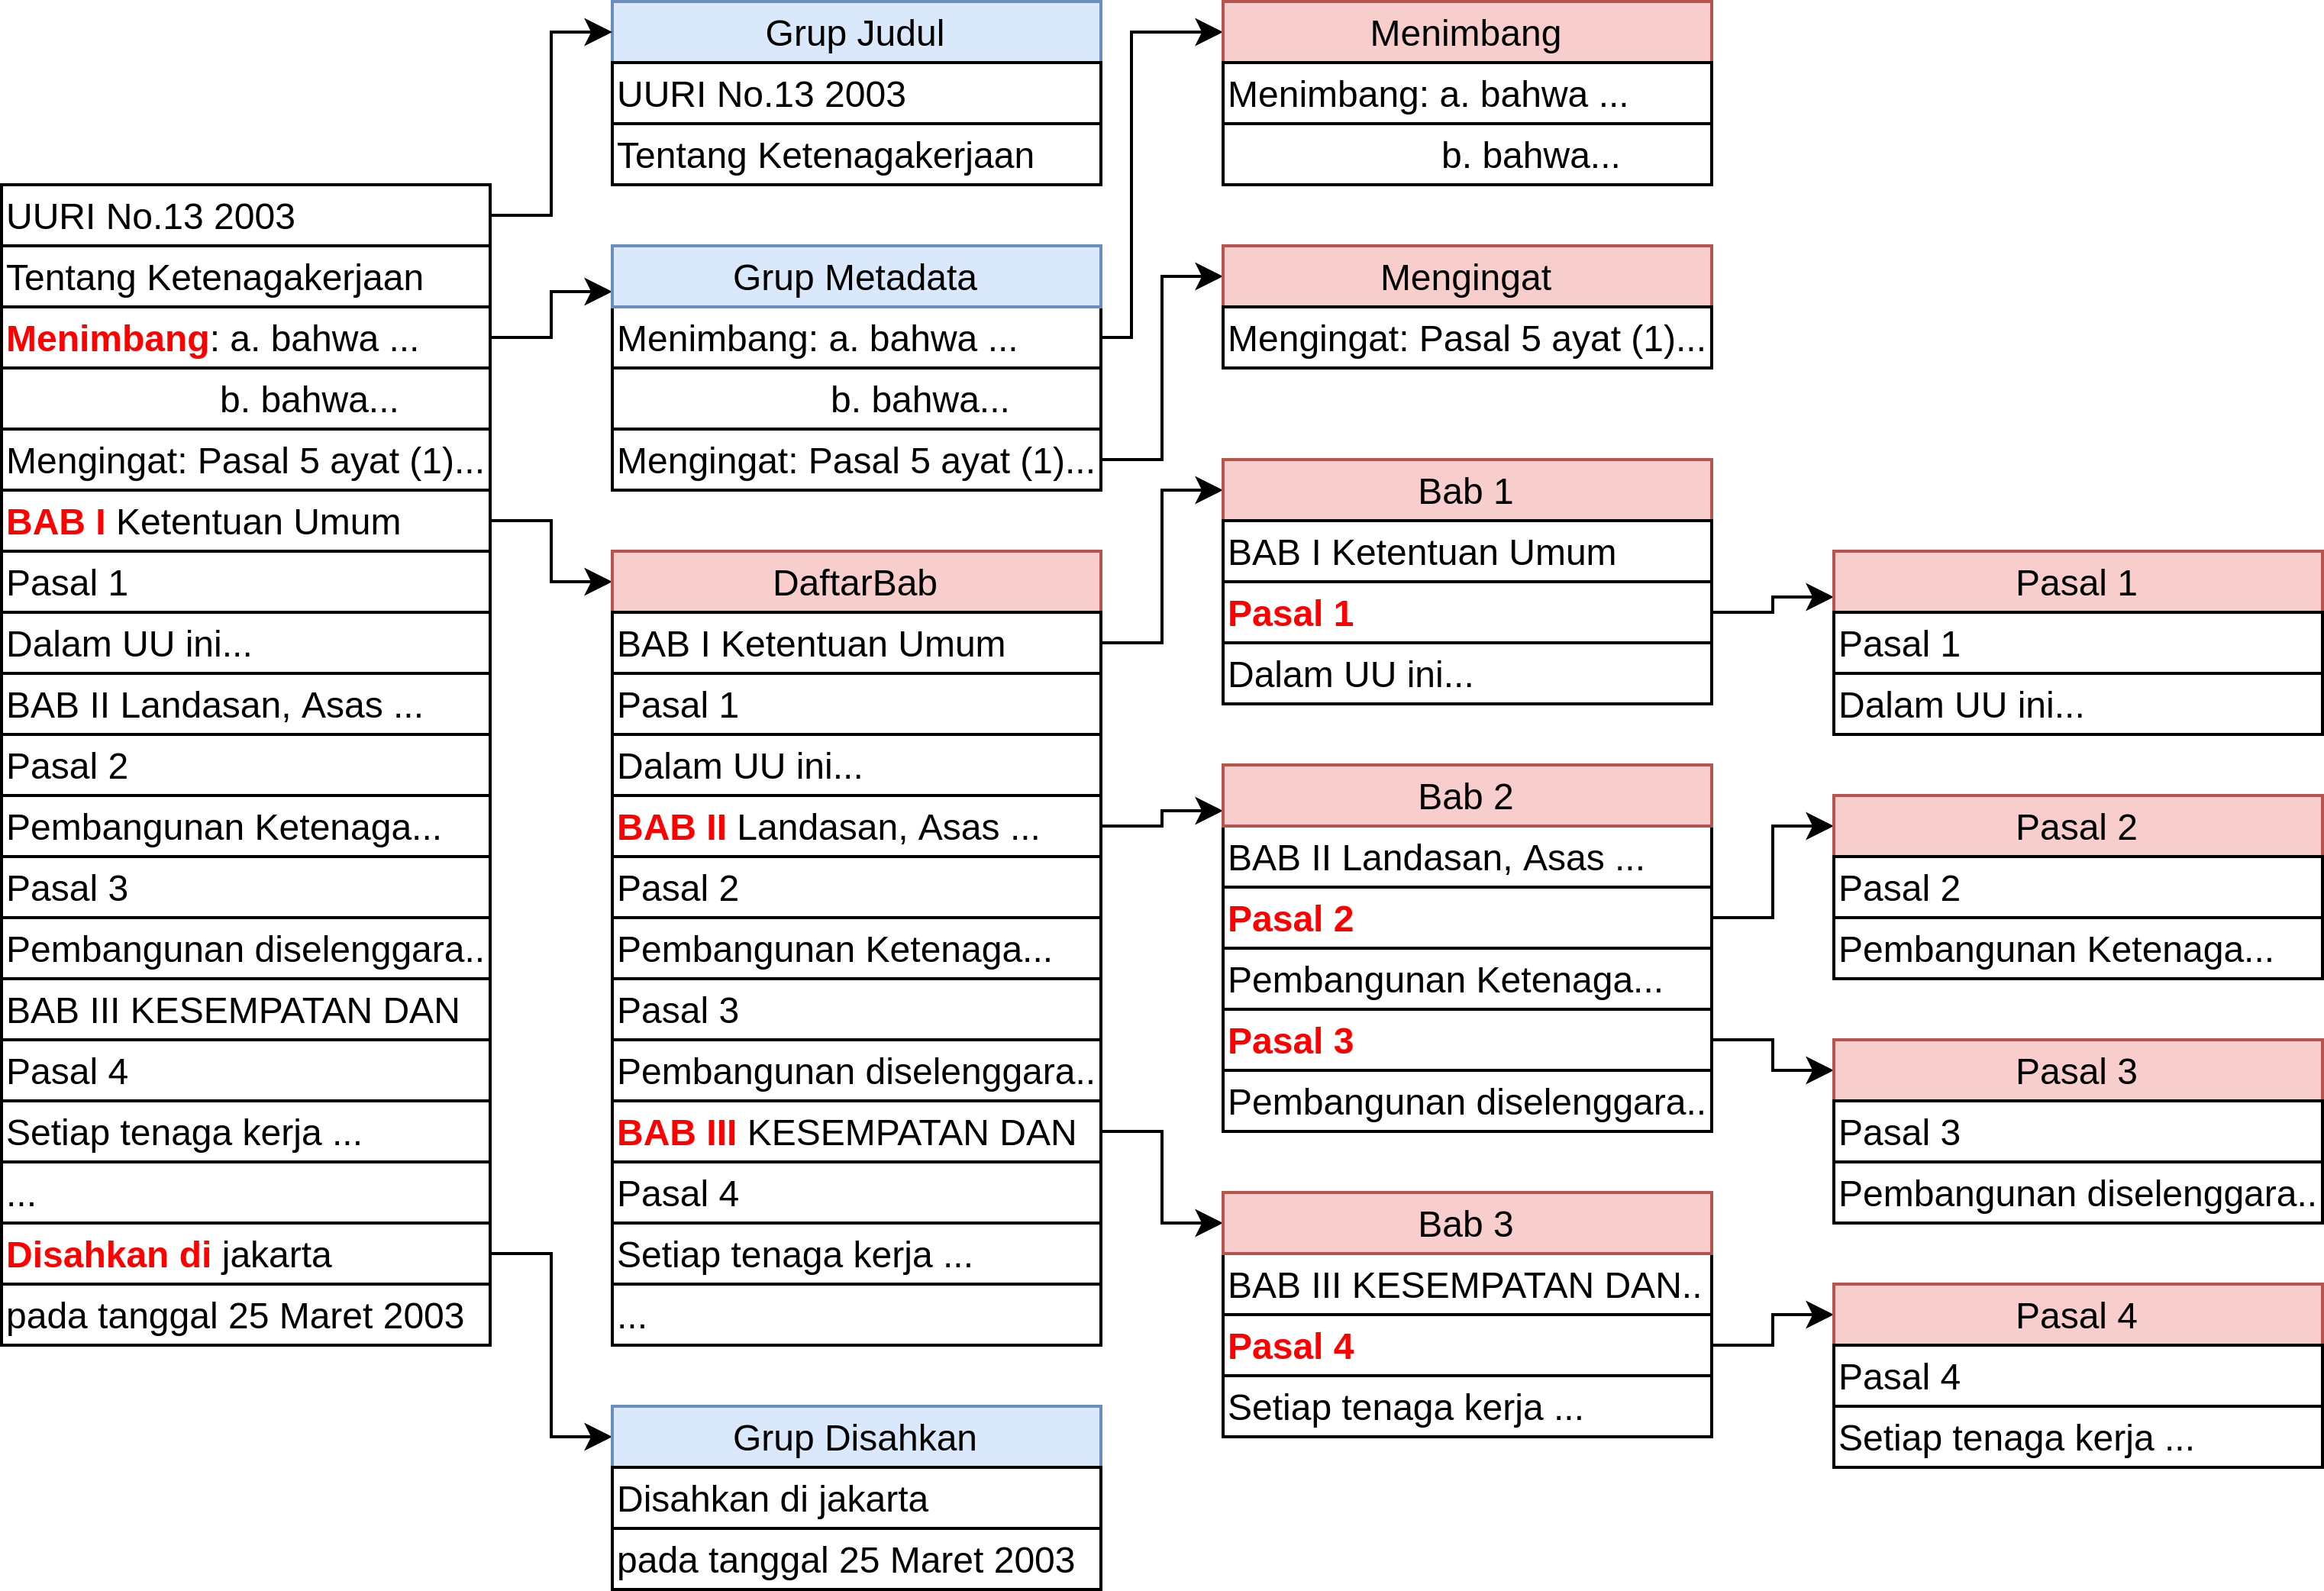
\includegraphics[width=\textwidth]{pictures/pdf_to_component.png}
  \caption{Ilustrasi Ekstraksi Daftar Span menjadi Data Struktur Komponen}
  \label{fig:ilustrasi-ekstraksi}
\end{figure}

Deteksi batas antara komponen atau grup dilakukan dengan melihat data pada \textit{span}
seperti \mono{str}, \mono{xL}, \mono{xR}, dan \mono{y}. Pada \pic~\ref{fig:ilustrasi-ekstraksi},
pola yang terdeteksi sebagai batas ditandai dengan \textcolor{red}{teks merah}. Sebagai contoh, pada
ekstraki paling kiri, dari daftar \textit{span} asli menjadi grup, dilakukan iterasi
\textit{span} dari atas dan akan dimasukkan ke dalam grup \textbf{Judul} sampai menemukan
grup yang diawali dengan kata \mono{Menimbang}. Kemudian setiap \textit{span} setelah
span \textbf{Menimbang} tersebut akan dikelompokkan menjadi grup \textbf{Metadata} sampai
menemukan grup yang diawali kata \mono{BAB I}.

%--------------------------------------------------------------------------------------------------%
\subsection{Komponen Terurut}
\label{subsec:komponen-terurut}
%--------------------------------------------------------------------------------------------------%

Beberapa komponen seperti \mono{o:Bab}, \mono{o:Bagian}, \mono{o:Paragraf}, \mono{o:Pasal}, dan
\mono{o:Huruf} memiliki sifat terurut. Dalam hal ini, yang dimaksud terurut adalah:

\begin{itemize}
  \item Komponen yang mengawali suatu komponen terurut akan selalu sama.
  \item Hanya terdapat satu komponen yang dapat mengikuti komponen terurut.
\end{itemize}

Contoh dari sifat pertama adalah \mono{o:Bab}, \mono{o:Bagian}, \mono{o:Paragraf}, dan
\mono{o:Pasal} pasti dimulai dari komponen nomor 1 seperti \mono{Bab 1} dan \mono{Pasal 1}, dan
\mono{o:Huruf} pasti dimulai dari komponen \mono{a.} atau \mono{1.}. Contoh dari sifat kedua
adalah hanya \mono{pasal 2} yang dapat mengikuti \mono{Pasal 1} dan hanya \mono{b.} yang dapat
mengikuti \mono{a.}. Dalam implementasi, penulis memastikan sifat-sifat ini dipatuhi, sehingga
sebagai contoh apabila sebuah dokumen terdeteksi mengandung \mono{Bab 12} maka akan dijamin
mengandung semua \mono{Bab 1} sampai \mono{Bab 11} dan apabila terdeteksi mengandung
\mono{Pasal 196} maka akan dijamin mengandung semua pasal dari \mono{Pasal 1} sampai
\mono{Pasal 195}.

%--------------------------------------------------------------------------------------------------%
\subsection{Komponen Amendemen}
\label{subsec:komponen-amendemen}
%--------------------------------------------------------------------------------------------------%

Melakukan \textit{parsing span} pada bagian amendemen merupakan salah satu tantangan pada penelitian
ini. \pic~\ref{fig:contoh-amendemen} adalah amendemen pada Pasal 17 UU 11/2020 yang dilakukan
terhadap Pasal 1 UU 26/2007. Dapat dilihat bahwa kata \mono{Pasal 17} dan \mono{Pasal 1} yang
digunakan sebagai pembatas antara komponen memiliki pola teks dan posisi yang hampir sama. Hal ini
membuat pembedaan antara ``Pasal biasa'' dan ``Pasal peng-amendemen'' menjadi sulit dilakukan.

\begin{figure}[H]
  \centering
  \fbox{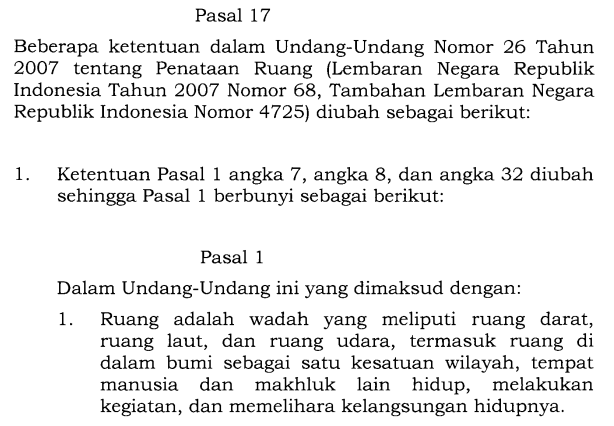
\includegraphics{pictures/pdf_amendment.png}}
  \caption{Contoh Amendemen pada UU 11/2020}
  \label{fig:contoh-amendemen}
\end{figure}

Untuk menyelesaikan masalah ini, penulis menggunakan koordinat \mono{xL} \textit{span} tepat
setelah \textit{span} yang bertuliskan ``Pasal X''. Pada contoh deteksi kompoonen amendemen
\pic~\ref{fig:deteksi-amendemen}, \mono{xL} dari teks setelah pasal peng-amendemen (pasal biasa)
ditandai dengan \textcolor{red}{lingkaran merah}, \mono{xL} dari pasal yang diamendemen ditandai
dengan \textcolor{blue}{lingkaran biru}, dan garis hijau merepresentasikan batas pembeda \mono{xL}
antara pasal biasa dan pasal yang diamendemen. Pembedaan pasal biasa dan pasal amendemen hanya
dilakukan jika dokumen memiliki komponen berupa amendemen.

\begin{figure}[H]
  \centering
  \fbox{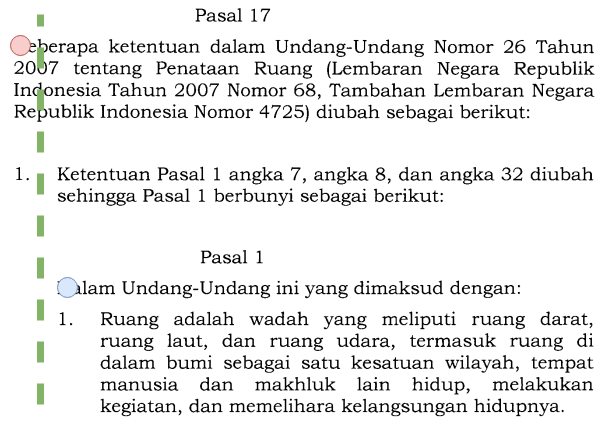
\includegraphics{pictures/amendment_detection.png}}
  \caption{Deteksi Komponen amendemen}
  \label{fig:deteksi-amendemen}
\end{figure}

%--------------------------------------------------------------------------------------------------%
\section{Deteksi Rujukan}
\label{sec:deteksi-rujukan}
%--------------------------------------------------------------------------------------------------%

Setelah semua \textit{span} dikelompokan menjadi suatu komponen, dilakukan deteksi rujukan pada teks
pada setiap komponen untuk mengetahui apakah komponen tersebut menyebut komponen atau dokumen \legal
lainnya. \tab~\ref{tab:rujukan} adalah daftar pola rujukan yang berhasil dideteksi pada penelitian
ini. Selain URI, data rujukan juga mengandung informasi seperti yang dijelaskan pada
\tab~\ref{tab:info-rujukan}. Contoh teks dan data rujukan yang terdeteksi dari teks tersebut dapat
dilihat pada \lst~\ref{lst:uu-13-2003-detect}.

\begin{table}
  \centering
  \begin{tabular}{|l|l|l|} \hline
    No.              & \multicolumn{2}{l|}{}                                                            \\ \hline \hline
    \multirow{4}*{1} & Pola                  & UUD 1945                                                 \\ \cline{2-3}
                     & Regex                 & \verb/Undang Undang Dasar Negara Republik Indonesia Tahun 1945/                               \\ \cline{2-3}
                     & Contoh teks           & Undang Undang Dasar Negara Republik Indonesia Tahun 1945 \\ \cline{2-3}
                     & URI                   & \texttt{:uud}                                            \\ \hline
    \hline
    \multirow{4}*{2} & Pola                  & Undang-Undang Nomor \{x\} Tahun \{y\}                    \\ \cline{2-3}
                     & Regex                 & \verb/Undang-Undang Nomor [0-9]+ Tahun [0-9]+/                               \\ \cline{2-3}
                     & Contoh teks           & Undang-Undang Nomor 26 Tahun 2007                        \\ \cline{2-3}
                     & URI                   & \texttt{:uu/2007/26}                                     \\ \hline
    \hline
    \multirow{4}*{3} & Pola                  & Pasal \{x\}                                              \\ \cline{2-3}
                     & Regex                 & \verb/Pasal [0-9]+/                               \\ \cline{2-3}
                     & Contoh teks           & Pasal 156                                                \\ \cline{2-3}
                     & URI                   & \texttt{:uu/2003/13/pasal/156}                           \\ \hline
    \hline
    \multirow{4}*{4} & Pola                  & ayat (\{x\})                                             \\ \cline{2-3}
                     & Regex                 & \verb/ayat \((l|[0-9]+)\)/                               \\ \cline{2-3}
                     & Contoh teks           & ayat (1)                                                 \\ \cline{2-3}
                     & URI                   & \texttt{:uu/2003/13/pasal/169/ayat/1}                    \\ \hline
    \hline
    \multirow{4}*{5} & Pola                  & Pasal \{x\} ayat (\{x\})                                 \\ \cline{2-3}
                     & Regex                 & \verb/Pasal [0-9]+ ayat \((l|[0-9]+)\)/                               \\ \cline{2-3}
                     & Contoh teks           & Pasal 156 ayat (2)                                       \\ \cline{2-3}
                     & URI                   & \texttt{:uu/2003/13/pasal/156/ayat/2}                    \\ \hline
    \hline
    \multirow{4}*{6} & Pola                  & huruf \{x\} dan huruf \{y\}                              \\ \cline{2-3}
                     & Regex                 & \verb/huruf ?([a-z]?,? ?)+( [a-z]( |,))/                               \\ \cline{2-3}
                     & Contoh teks           & huruf a dan b                                            \\ \cline{2-3}
                     & \multirow{2}*{URI}    & \texttt{uu/2003/13/pasal/1/point/5/point/a}              \\ \cline{3-3}
                     &                       & \texttt{uu/2003/13/pasal/1/point/5/point/b}              \\ \hline
    \hline
    \multirow{4}*{7} & Pola                  & huruf \{x\}, \{y\}, ... dan \{z\}                        \\ \cline{2-3}
                     & Regex                 & \verb/huruf ?([a-z]?,? ?)+( [a-z]( |,))/                               \\ \cline{2-3}
                     & Contoh teks           & huruf a, b, c, d, dan e                                  \\ \cline{2-3}
                     & \multirow{5}*{URI}    & \texttt{uu/2003/13/menimbang/point/a}                    \\ \cline{3-3}
                     &                       & \texttt{uu/2003/13/menimbang/point/b}                    \\ \cline{3-3}
                     &                       & \texttt{uu/2003/13/menimbang/point/c}                    \\ \cline{3-3}
                     &                       & \texttt{uu/2003/13/menimbang/point/d}                    \\ \cline{3-3}
                     &                       & \texttt{uu/2003/13/menimbang/point/e}                    \\ \hline
  \end{tabular}
  \caption{Pola, contoh teks, dan contoh URI deteksi rujukan}
  \label{tab:rujukan}
\end{table}

\begin{table}
  \centering
  \begin{tabular}{|l|l|} \hline
    Nama           & Deskripsi                             \\\hline \hline
    \texttt{start} & \textit{index} karakter awal rujukan  \\\hline
    \texttt{end}   & \textit{index} karakter akhir rujukan \\\hline
    \texttt{uri}   & URI dokumen dan                       \\\hline
  \end{tabular}
  \caption{Data rujukan}
  \label{tab:info-rujukan}
\end{table}

\begin{listing}[H]
  \begin{minted}[fontsize=\scriptsize, frame=single]{yaml}
textString: >-
  Pekerja/buruh yang diputus hubungan kerjanya berdasarkan alasan
  sebagaimana dimaksud dalam ayat (1), dapat memperoleh uang
  penggantian hak sebagaimana dimaksud dalam Pasal 156 ayat (4).
references:
  - start: 91
    end: 99
    uri: /uu/2003/13/pasal/158/ayat/1
  - start: 166
    end: 184
    uri: /uu/2003/13/pasal/156/ayat/4
  \end{minted}
  \caption{Contoh teks pada Pasal 158 Ayat (4) UU 13/2003 beserta rujukan yang terdeteksi}
  \label{lst:uu-13-2003-detect}
\end{listing}

Untuk melakukan deteksi, teks akan melalui fungsi yang masing-masing memiliki pola untuk dideteksi.
Oleh karena itu, untuk \textit{substring} yang beririsan dapat memiliki lebih dari dua rujukan yang
terdeteksi. Pada kasus tersebut akan diambil rujukan dengan \textit{substring} terpanjang. Sebagai
contoh, teks ``Pasal 156 Ayat (4)'' pada UU No.13 Tahun 2003 Pasal 158 Ayat (4) akan terdeteksi
sebagai 3 URI rujukan seperti yang terlihat pada \tab~\ref{tab:contoh-teks-uri}. Pada kasus ini,
yang akan diambil adalah teks ``Pasal 156 ayat (4)'' karena merupakan teks terpanjang.

\begin{table}
  \centering
  \begin{tabular}{|l|l|} \hline
    Teks               & URI                                   \\\hline \hline
    Pasal 156 Ayat (4) & \texttt{/uu/2003/13/pasal/156/ayat/4} \\\hline
    Pasal 156          & \texttt{/uu/2003/13/pasal/156}        \\\hline
    Ayat (4)           & \texttt{/uu/2003/13/pasal/158/ayat/4} \\\hline
  \end{tabular}
  \caption{Contoh teks dan URI yang terdeteksi dari teks tersebut}
  \label{tab:contoh-teks-uri}
\end{table}


%--------------------------------------------------------------------------------------------------%
\section{Konstruksi KG}
\label{data-to-triple}
%--------------------------------------------------------------------------------------------------%

\begin{figure}
  \centering
  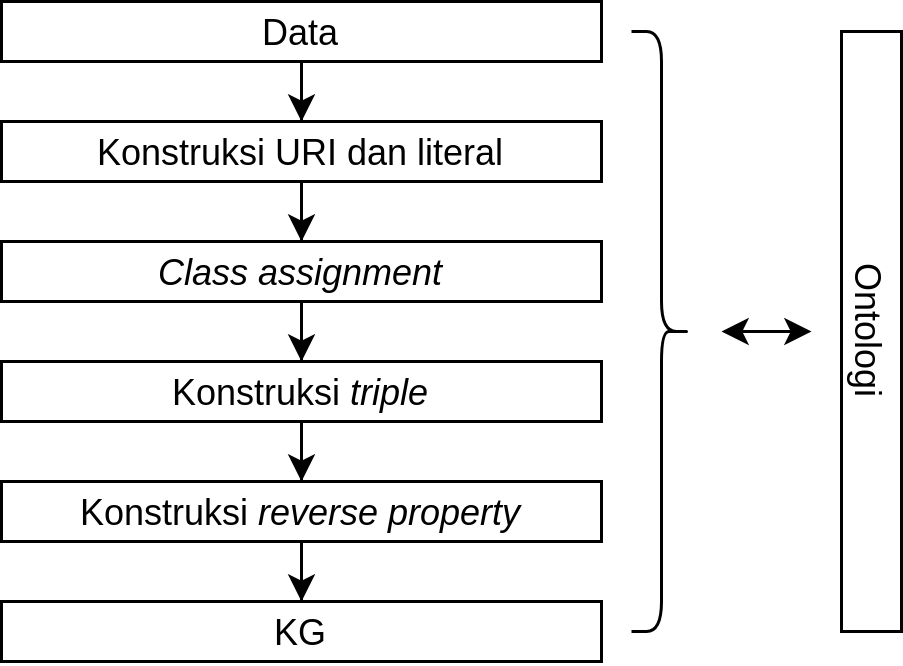
\includegraphics[scale=0.4]{pictures/konstruksi_kg.png}
  \caption{Konstruksi KG}
  \label{fig:konstruksi-kg}
\end{figure}

Seluruh proses konstruksi KG didasari dengan ontologi yang sudah dirancang pada bab sebelumnya. KG
dikonstruksi dari data \legal yang sudah terdapat sebagai data terstruktur dalam memori. Setiap
objek seperti peraturan dan komponen akan dibangun menjadi URI berdasarkan
\tab~\ref{tab:uri-peraturan} dan \tab~\ref{tab:uri-peraturan}. Literal seperti bilangan,
\textit{string}, dan tanggal juga dikonversi sesuai spesifikasi \textit{literal type} pada Turtle.
Setiap objek juga akan di-\textit{assign} ke masing-masing \textit{class} sesuai yang terdapat pada
\tab~\ref{tab:class}. Kemudian \textit{triple} dibangun berdasarkan relasi antara peraturan atau
komponen dengan properti, domain, dan range sesuai spesifikasi pada \tab~\ref{tab:properti}. Untuk
setiap properti struktur, akan dibuat \textit{reverse property} nya yaitu \mono{o:bagianDari}.
Sebagai contoh, jika terdapat \textit{triple} \mono{uu:2020/11/bab o:bab uu:2020/11/bab/1},
\textit{reverse triple} nya adalah \mono{uu:2020/11/bab/1 o:bab uu:2020/11/bab}. Properti struktur
antaralain adalah \mono{o:ayat}, \mono{o:bab}, \mono{o:bagian}, \mono{o:daftarAyat},
\mono{o:daftarBab}, \mono{o:daftarBagian}, \mono{o:daftarHuruf}, \mono{o:daftarParagraf},
\mono{o:daftarPasal}, \mono{o:huruf}, \mono{o:paragraf}, \mono{o:pasal}, \mono{o:segmen},
\mono{o:teks}, dan \mono{o:versi}.


%--------------------------------------------------------------------------------------------------%
\section{Query}
\label{sec:query}
%--------------------------------------------------------------------------------------------------%

\textit{Query} dilakukan terhadap KG untuk evaluasi \textit{competency question} dan membuat
demonstrasi untuk \textit{use case evaluation}. Apache Jena
Fuseki\footnote{\url{https://jena.apache.org/documentation/fuseki2/}} digunakan sebagai SPARQL
server yang menyimpan KG dan melakukan \textit{query} terhadap KG. Di dalam folder Fuseki, Fuseki
dapat dijalankan dengan KG yang memuat berkas Turtle \mono{lex2kg.ttl} dan memiliki endpoint SPARQL
\textit{/lex2kg} dengan \lst~\ref{lst:run-fuseki}. Setelah command tersebut dijalankan, SPARQL
\textit{query} dapat dilakukan menggunakan \textit{client library} dengan endpoint
\url{http://127.0.0.1:3030/lex2kg/sparql}, atau pada antarmuka yang tersedia pada
\url{http://127.0.0.1:3030/dataset.html?tab=query&ds=/lex2kg}. Pada penelitian ini digunakan
\textit{client library}
\texttt{fetch-sparql-endpoint}\footnote{\url{https://www.npmjs.com/package/fetch-sparql-endpoint}}
untuk melakukan \textit{query} dari bahasa pemrograman typescript.


\begin{listing}[H]
  \begin{minted}[fontsize=\scriptsize, frame=single, breaklines]{bash}
java -jar fuseki-server.jar --file=lex2kg.ttl /lex2kg
  \end{minted}
  \caption{Command untuk menjalankan Fuseki}
  \label{lst:run-fuseki}
\end{listing}

%--------------------------------------------------------------------------------------------------%
\section{Konversi Skala Besar}
\label{sec:konversi-skala-besar}
%--------------------------------------------------------------------------------------------------%

Penulis melakukan konversi skala besar pada PDF UU yang terdapat pada Laman Undang-Undang Jaringan
Dokumentasi dan Informasi Hukum DPR RI.\footnote{\url{https://www.dpr.go.id/jdih/uu}} Dari 1669
berkas PDF yang diunduh, 784 diantaranya berhasil dikonversi menjadi KG dengan total 1.163.051
\textit{triple}. Jumlah tripel dikelompokan berdasarkan jenis informasi dapat dilihat pada
\tab~\ref{tab:analisis-triple}. Semua berkas PDF, berkas Turtle hasil konversi, dan berkas
\textit{artifact} seperti PDF hasil OCR, dan \textit{span} dari konversi skala besar dapat diakses
pada repositori \url{https://github.com/aabccd021/uuri}.

\begin{table}
  \centering
  \begin{tabular}{|l|l|} \hline
    Jenis Informasi           & Jumlah Triple \\\hline \hline
    metadata peraturan        & 6.689         \\\hline
    struktur peraturan        & 714.888       \\\hline
    teks                      & 152.301       \\\hline
    rujukan dan amendemen     & 32.577        \\\hline
    \textit{class assignment} & 256.416       \\\hline
  \end{tabular}
  \caption{Analisis \textit{triple} KG hasil konversi skala besar}
  \label{tab:analisis-triple}
\end{table}

%--------------------------------------------------------------------------------------------------%
\section{Hasil Konversi}
\label{sec:hasil-konversi}
%--------------------------------------------------------------------------------------------------%

\lst~\ref{lst:res} merupakan contoh \textit{subset} KG UU 8/2020 tentang Pertanggungjawaban atas
pelaksanaan APBN yang dihasilkan oleh Lex2KG. Dapat dilihat bahwa UU 8/2020 dilengkapi dengan
metadata yang diekstraksi dari PDF, dilengkapi dengan \textit{class assignment} \mono{a
o:Peraturan}, dan diberi jenis peraturan sesuai \textit{resource} pada ontologi yaitu \mono{jp:UU}.
Struktur peraturan berupa menimbang dan teks juga terdapat dalam KG tersebut. \textit{Teverse
property} dari \mono{o:teks} juga dikonstruksi yaitu \mono{o:bagianDari}. \textit{Reverse property}
dari \mono{o:teks} dan \mono{o:huruf} juga dikonstruksi yaitu \mono{o:bagianDari}. Pertimbangan UU
8/2020 terhadap UU 12/2018 juga berhasil diekspresikan daadaplam bentuk rujukan pada komponen
\mono{o:Menimbang}.

\begin{listing}[H]
  \begin{minted}[fontsize=\scriptsize, frame=single, breaklines]{turtle}
@prefix o: <https://example.org/lex2kg/ontology/> .
@prefix jp: <https://example.org/lex2kg/jenisPeraturan/> .

<https://example.org/lex2kg/uu/2020/8>
    a o:Peraturan ;
    o:yurisdiksi "Indonesia";
    o:jenisPeraturan jp:UU;
    o:tahun 2020;
    o:bahasa "id";
    o:tentang " CIPTA KERJA";
    o:disahkanPada "2020-11-02"^^xsd:date;
    o:disahkanDi "Jakarta";
    o:disahkanOleh "JOKO WIDODO";
    o:jabatanPengesah "PRESIDEN REPUBLIK INDONESIA,";
    o:menimbang <https://example.org/lex2kg/uu/2020/8/menimbang> .

<https://example.org/lex2kg/uu/2020/8/menimbang> 
    o:huruf <https://example.org/lex2kg/uu/2020/8/menimbang/huruf/b> .

<https://example.org/lex2kg/uu/2020/8/menimbang/huruf/b> 
    o:bagianDari <https://example.org/lex2kg/uu/2020/8/menimbang> ;
    o:teks <https://example.org/lex2kg/uu/2020/8/menimbang/huruf/b/text> .

<https://example.org/lex2kg/uu/2020/8/menimbang/huruf/b/text> 
    o:bagianDari <https://example.org/lex2kg/uu/2020/8/menimbang/huruf/b> ;
    o:merujuk <https://example.org/lex2kg/uu/2018/12> .

  \end{minted}
  \caption{Contoh KG UU Cipta Kerja}
  \label{lst:res}
\end{listing}

